\documentclass[12pt]{article}
\usepackage{graphicx}
%\documentclass[journal,12pt,twocolumn]{IEEEtran}
\usepackage[none]{hyphenat}
\usepackage{graphicx}
\usepackage{listings}
\usepackage[english]{babel}
\usepackage{graphicx}
\usepackage{caption} 
\usepackage{hyperref}
\usepackage{booktabs}
\usepackage{commath}
\usepackage{gensymb}
\usepackage{array}
\usepackage{amsmath}   % for having text in math mode
\usepackage{listings}
\lstset{
  frame=single,
  breaklines=true
}
  
%Following 2 lines were added to remove the blank page at the beginning
\usepackage{atbegshi}% http://ctan.org/pkg/atbegshi
\AtBeginDocument{\AtBeginShipoutNext{\AtBeginShipoutDiscard}}
%


%New macro definitions
\newcommand{\mydet}[1]{\ensuremath{\begin{vmatrix}#1\end{vmatrix}}}
\providecommand{\brak}[1]{\ensuremath{\left(#1\right)}}
\providecommand{\norm}[1]{\left\lVert#1\right\rVert}
\newcommand{\solution}{\noindent \textbf{Solution: }}
\newcommand{\myvec}[1]{\ensuremath{\begin{pmatrix}#1\end{pmatrix}}}
\let\vec\mathbf


\begin{document}
\begin{center}
\title{\textbf{chapter-11}}
\date{\vspace{-5ex}} %Not to print date automatically
\maketitle
\end{center}
\setcounter{page}{1}
\section{Exercise 10.4.7}

\begin{enumerate}
\item Find the equation of line  drawn perpendicular to the line $\frac{x}{4}+\frac{y}{6}=1$ through the point where it meets the y-axis \\
\section{Solution} The given equation can be arranged as
\begin{align}
3x+2y-12&=0 \label{eq:1}
\end{align}
The \eqref{eq:1} can be expressed as  
\begin{align}
	\vec{n}^{\top}\vec{x}=c
\end{align}
\begin{align}
	\text{ where }
		\vec{n} = \myvec{3\\2}, c=12 
\end{align}
the equation of line perpendicular where it meets $y$-axis through point(0,6)
\begin{align}
	\vec{m}^\top\brak{\vec{x}-\vec{A}}=0\label{eq:5}
\end{align}
		where $\vec{A}$ and $\vec{m}$ is 
\begin{align}
	\vec{m}^{\top} &=\myvec{-2 & 3}\\
	\vec{A} &=\myvec{0\\6}
\end{align}
Substituting the value of $\vec{m}$ and $\vec{A}$ in \eqref{eq:5}
		\begin{align}
			\myvec{-2 & 3}\brak{\vec{x}-\myvec{0\\6}} &=0\\
			\myvec{-2 & 3}\vec{x} &=-18
		\end{align}
\begin{figure}[h]
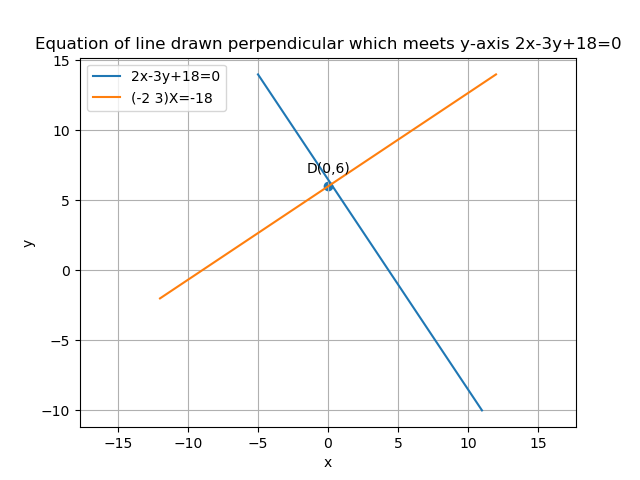
\includegraphics[width=\columnwidth]{figs/fig.png}
\caption{}
  \label{fig:Figure}
\end{figure}
\end{enumerate}
\end{document}